% =============================================================================
%  FIVUCSAS — Poster variant: DARK CYBERPUNK
%  A0 portrait. Black background, neon cyan/magenta/green, monospace headings.
%  Compile:  pdflatex poster.tex && pdflatex poster.tex
% =============================================================================
\documentclass[a0paper,portrait]{tikzposter}
\tikzposterlatexaffectionproofoff
\geometry{paperwidth=841mm,paperheight=1189mm}

\usepackage[utf8]{inputenc}
\usepackage[T1]{fontenc}
\usepackage{lmodern}
\usepackage{microtype}
\usepackage{xcolor}
\usepackage{graphicx}
\graphicspath{{../../assets/}{./assets/}{./poster/assets/}}
\usepackage{eso-pic}
\usepackage{fontawesome5}
\usepackage{qrcode}
\usepackage{tikz}
\usepackage{enumitem}
\usepackage{array}
\usetikzlibrary{positioning,calc,arrows.meta,backgrounds,decorations.pathreplacing,fadings}

% Official institutional crests (assets/)
\newcommand{\unicrest}[1][2.6cm]{
\includegraphics[height=#1,keepaspectratio]{marmara-university.png}}
\newcommand{\faccrest}[1][2.6cm]{
\includegraphics[height=#1,keepaspectratio]{muhendislik-fakultesi.jpg}}

% ---------- Cyberpunk palette ------------------------------------------------
\definecolor{CBg}{HTML}{05070D}        % near-black
\definecolor{CPanel}{HTML}{0C1322}     % panel
\definecolor{CPanelLite}{HTML}{14203A} % lighter panel
\definecolor{CInk}{HTML}{E6F0FF}       % ice white
\definecolor{CDim}{HTML}{6B7C99}       % dim gray-blue
\definecolor{CCyan}{HTML}{00E5FF}      % neon cyan
\definecolor{CMagenta}{HTML}{FF1F8F}   % neon magenta
\definecolor{CGreen}{HTML}{00FF99}     % terminal green
\definecolor{CGold}{HTML}{FFC857}      % warning gold
\definecolor{CGrid}{HTML}{1A2940}      % subtle grid

% ---------- Theme ------------------------------------------------------------
\definelayouttheme{Cyber}{
  \usecolorstyle[colorPalette=CyberPal]{Default}
  \usebackgroundstyle{Empty}
  \usetitlestyle{Empty}
  \useblockstyle{Empty}
  \useinnerblockstyle{Default}
  \usenotestyle{Default}
}
\definecolorpalette{CyberPal}{
  \definecolor{colorOne}{named}{CBg}
  \definecolor{colorTwo}{named}{CPanel}
  \definecolor{colorThree}{named}{CCyan}
}
\usetheme{Cyber}
\colorlet{backgroundcolor}{CBg}
\colorlet{framecolor}{CBg}
\colorlet{titlefgcolor}{CCyan}
\colorlet{titlebgcolor}{CBg}
\colorlet{blocktitlebgcolor}{CBg}
\colorlet{blocktitlefgcolor}{CCyan}
\colorlet{blockbodybgcolor}{CBg}
\colorlet{blockbodyfgcolor}{CInk}
\colorlet{innerblocktitlebgcolor}{CCyan}
\colorlet{innerblocktitlefgcolor}{CBg}

% Background is overridden in-document via a remember-picture overlay that
% paints the whole page CBg and lays down the subtle grid. tikzposter's own
% backgroundstyle remains "Empty" so it does not draw a default rectangle.

% ---------- Neon glow node helper -------------------------------------------
\newcommand{\neonbox}[2]{%
  \begin{tikzpicture}
    \node[draw=#1, line width=0.6pt, fill=CPanel, rounded corners=2pt,
          inner sep=6pt, font=\ttfamily\bfseries, text=#1] {#2};
  \end{tikzpicture}%
}

\newcommand{\hudtile}[3]{% color, icon, label
  \begin{tikzpicture}[baseline=(b.center)]
    \node[draw=#1, line width=0.5pt, fill=CPanel, text=#1,
          rounded corners=2pt, minimum width=3.4cm, minimum height=2.6cm,
          align=center, font=\ttfamily\bfseries, inner sep=2pt] (b)
      {{\fontsize{22}{24}\selectfont #2}\\[1pt]{\small #3}};
  \end{tikzpicture}}

% ---------- Title ------------------------------------------------------------
\title{\parbox{0.96\linewidth}{\centering\ttfamily
  \begin{minipage}[c]{0.11\linewidth}\centering
    \fcolorbox{CCyan}{white}{\unicrest[2.0cm]}
  \end{minipage}\hfill
  \begin{minipage}[c]{0.74\linewidth}\centering\ttfamily
  {\fontsize{72}{72}\selectfont\bfseries\color{CCyan}FIVUCSAS}\\[0.1em]
  {\color{CMagenta}\rule{0.6\linewidth}{1.5pt}}\\[0.2em]
  {\large\color{CInk}\textsc{Face and Identity Verification :: Cloud-based SaaS}}\\[0.2em]
  {\small\color{CGreen}> multi\_tenant\_biometric\_auth.sys --active-liveness --anti-spoof}
  \end{minipage}\hfill
  \begin{minipage}[c]{0.11\linewidth}\centering
    \fcolorbox{CMagenta}{white}{\faccrest[2.2cm]}
  \end{minipage}
}}
\author{}
\institute{}

% Force-black page background via eso-pic shipout hook so it does NOT
% reserve any vertical layout space (the prior in-document
% `tikzpicture[overlay]` form pushed the title block off the page).
\AddToShipoutPictureBG{%
  \AtPageLowerLeft{\color{CBg}\rule{\paperwidth}{\paperheight}}%
  \AtPageLowerLeft{\begin{tikzpicture}[remember picture]
    \foreach \x in {0,4,...,84}{\draw[CGrid, line width=0.2pt] (\x,0) -- (\x,119);}
    \foreach \y in {0,4,...,119}{\draw[CGrid, line width=0.2pt] (0,\y) -- (84,\y);}
  \end{tikzpicture}}}

\begin{document}
\maketitle[width=\paperwidth, titletotopverticalspace=10mm]

% Authors strip ---------------------------------------------------------------
\block[bodyoffsety=-20mm, bodyinnersep=2mm]{}{\centering\ttfamily\color{CDim}\small
> authors[] = \{\textcolor{CInk}{Ahmet Abdullah Gültekin},\ \textcolor{CInk}{Ayşe Gülsüm Eren},\ \textcolor{CInk}{Ayşenur Arıcı}\}\\
> advisor    = \textcolor{CInk}{Mustafa Ağaoğlu}\quad course = \textcolor{CInk}{CSE4197 / CSE4198}\quad term = \textcolor{CInk}{Spring 2025-2026}\\
> institution = \textcolor{CInk}{Marmara University · Faculty of Engineering · Department of Computer Engineering}
}

% =============================================================================
% KPI HUD STRIP
% =============================================================================
\block[bodyoffsety=-2mm, bodyinnersep=4mm]{}{\centering
\begin{tikzpicture}[every node/.style={align=center}]
  % brackets around each KPI for HUD feel
  \foreach \cx/\val/\lbl/\sub in {%
    -18/0\%/{REPLAY\_FAR}/{n=120 recorded-video attempts},
      0/<1s/{E2E\_LATENCY}/{P95 = 950ms, CPU only},
     18/10/{AUTH\_FACTORS}/{face + voice + NFC + WebAuthn + ...}}{
    \draw[CCyan, line width=0.6pt] (\cx-5.5,1.6) -- (\cx-5.0,1.6) -- (\cx-5.0,2.0);
    \draw[CCyan, line width=0.6pt] (\cx+5.5,1.6) -- (\cx+5.0,1.6) -- (\cx+5.0,2.0);
    \draw[CCyan, line width=0.6pt] (\cx-5.5,-2.0) -- (\cx-5.0,-2.0) -- (\cx-5.0,-2.4);
    \draw[CCyan, line width=0.6pt] (\cx+5.5,-2.0) -- (\cx+5.0,-2.0) -- (\cx+5.0,-2.4);
    \node[font=\fontsize{42}{42}\selectfont\ttfamily\bfseries, text=CCyan] at (\cx,0)    {\val};
    \node[font=\ttfamily\small,    text=CMagenta]                    at (\cx,-1.2) {[\lbl]};
    \node[font=\footnotesize,      text=CDim,  align=center]         at (\cx,-2.0) {\sub};
  }
  \node[font=\ttfamily\small, text=CGreen] at (-9,2.4) {//};
  \node[font=\ttfamily\small, text=CGreen] at ( 9,2.4) {//};
\end{tikzpicture}}

% =============================================================================
% COLUMNS
% =============================================================================
\begin{columns}

% --------------- LEFT --------------------------------------------------------
\column{0.34}

\block{\ttfamily [01] PROBLEM}{%
\color{CInk}\small Online authentication is fragmented. Passwords leak,
SMS OTPs are SIM-swappable, hardware keys exclude phone-only users, and most
biometric services trust a \textcolor{CMagenta}{\bfseries single passive signal}
— a still selfie or a recorded clip — that a prepared attacker can replay.

\vspace{0.4em}
GDPR / KVKK demand verifiable consent, the right to erasure, and data
portability; consumer auth stacks treat these as an afterthought.

\vspace{0.4em}
\textcolor{CCyan}{\ttfamily\bfseries > goal:} a tenant-configurable, multi-modal
identity platform where any subset of \textcolor{CGreen}{\bfseries 10} factors
composes into MFA flows, and every biometric factor is protected by an
\emph{active}, randomised liveness challenge a recorded video cannot replay.}

\block{\ttfamily [02] SYSTEM TOPOLOGY}{%
\centering
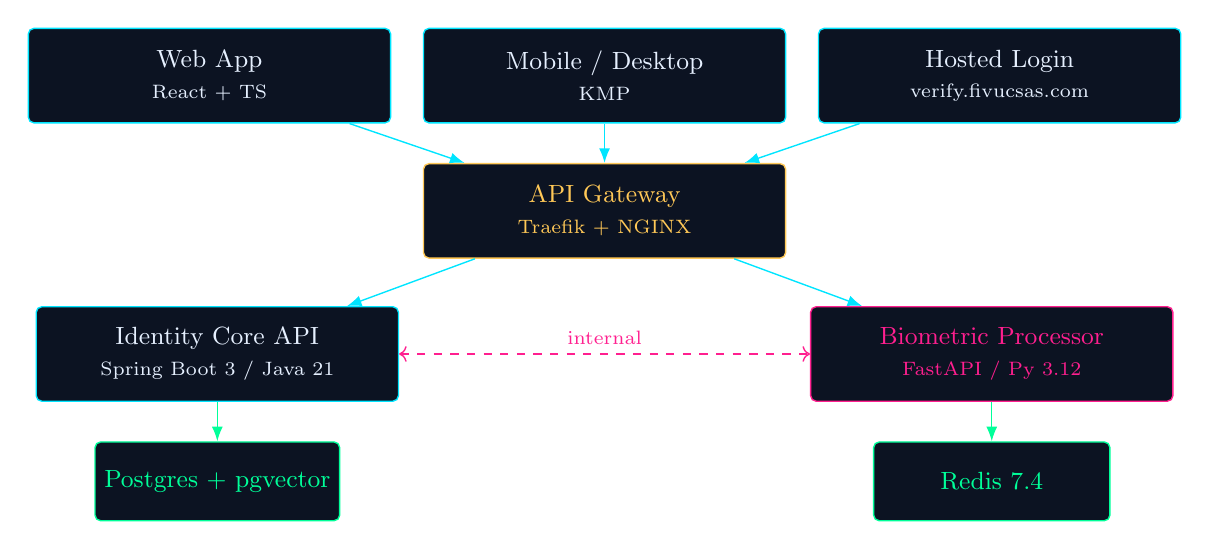
\begin{tikzpicture}[every node/.style={font=\small, text=CInk},
  svc/.style ={draw=CCyan, line width=0.5pt, fill=CPanel, rounded corners=2pt,
               minimum width=4.6cm, minimum height=1.2cm, align=center, text=CInk},
  ml/.style  ={draw=CMagenta, line width=0.5pt, fill=CPanel, rounded corners=2pt,
               minimum width=4.6cm, minimum height=1.2cm, align=center, text=CMagenta},
  data/.style={draw=CGreen, line width=0.5pt, fill=CPanel, rounded corners=2pt,
               minimum width=3.0cm, minimum height=1.0cm, align=center, text=CGreen},
  arrow/.style={-Latex, draw=CCyan, line width=0.5pt}]
\node[svc] (web)     {Web App\\\scriptsize React + TS};
\node[svc, right=4mm of web]    (mobile) {Mobile / Desktop\\\scriptsize KMP};
\node[svc, right=4mm of mobile] (widget) {Hosted Login\\\scriptsize verify.fivucsas.com};
\node[svc, below=5mm of mobile, draw=CGold, text=CGold] (gw) {API Gateway\\\scriptsize Traefik + NGINX};
\node[svc, below left=6mm and 0.3cm of gw] (api) {Identity Core API\\\scriptsize Spring Boot 3 / Java 21};
\node[ml,  below right=6mm and 0.3cm of gw] (bio) {Biometric Processor\\\scriptsize FastAPI / Py 3.12};
\node[data, below=5mm of api]  (db)   {Postgres + pgvector};
\node[data, below=5mm of bio]  (redis){Redis 7.4};
\foreach \src in {web,mobile,widget} {\draw[arrow] (\src) -- (gw);}
\draw[arrow] (gw) -- (api); \draw[arrow] (gw) -- (bio);
\draw[arrow, draw=CGreen] (api) -- (db); \draw[arrow, draw=CGreen] (bio) -- (redis);
\draw[arrow,<->,dashed, draw=CMagenta] (api) -- node[above,sloped,font=\scriptsize,text=CMagenta]{internal} (bio);
\end{tikzpicture}\par\vspace{1mm}
{\small\ttfamily\color{CDim}// biometric svc: no public route. docker net + api-key gated.}}

\block{\ttfamily [03] PASSIVE \texttt{||} ACTIVE LIVENESS}{%
\centering
\begin{tikzpicture}[every node/.style={font=\small, align=center}]
  \node[fill=CPanel, draw=CMagenta, line width=0.6pt, rounded corners=2pt,
        minimum width=8.8cm, minimum height=5.0cm,
        text width=8.2cm, anchor=north west, text=CInk] (p) at (-9.2,2)
    {\ttfamily\bfseries\textcolor{CMagenta}{[PASSIVE\_ONLY]}\\[2pt]
     \footnotesize\raggedright single frame -> texture / colour cues.\\
     \footnotesize\textcolor{CMagenta}{\faTimes}\ photo of phone screen \textit{often passes}\\
     \footnotesize\textcolor{CMagenta}{\faTimes}\ recorded clip \textit{passes}\\
     \footnotesize\textcolor{CMagenta}{\faTimes}\ deepfake injection \textit{often passes}};
  \node[fill=CPanel, draw=CGreen, line width=0.6pt, rounded corners=2pt,
        minimum width=8.8cm, minimum height=5.0cm,
        text width=8.2cm, anchor=north west, text=CInk] (a) at (0.4,2)
    {\ttfamily\bfseries\textcolor{CGreen}{[ACTIVE\_CHALLENGE]}\\[2pt]
     \footnotesize\raggedright n-step facial-action sequence + landmark verification + passive layer.\\
     \footnotesize\textcolor{CGreen}{\faCheck}\ photo \textit{fails}\\
     \footnotesize\textcolor{CGreen}{\faCheck}\ recorded clip \textit{fails (sequence mismatch)}\\
     \footnotesize\textcolor{CGreen}{\faCheck}\ deepfake \textit{must hit cues live}};
\end{tikzpicture}}

% --------------- MIDDLE ------------------------------------------------------
\column{0.32}

\block{\ttfamily [04] CONTRIBUTIONS}{%
\color{CInk}\small
\begin{enumerate}[leftmargin=*, nosep, label=\textcolor{CCyan}{\ttfamily\bfseries [C\arabic*]}, itemsep=3pt]
  \item \textbf{Tenant-configurable composition} of 10 auth factors into MFA flows declared at admin layer.
  \item \textbf{Active randomised liveness} — n-step facial-action sequence bound to per-attempt nonce, server-verified.
  \item \textbf{Pipeline decomposition} along OIDC-contract / ML-iteration boundary into two services on a private Docker network.
  \item \textbf{Embedding-at-rest encryption} — Facenet512 wrapped in Fernet (AES-128-CBC + HMAC-SHA-256) prior to pgvector write.
  \item \textbf{Regulator-aware data lifecycle} — tenant-scoped soft-delete + scheduled purge + audit logs (GDPR Art.\,15/17, KVKK).
\end{enumerate}}

\block{\ttfamily [05] METHODS}{%
\color{CInk}\small
Monolithic auth was rejected early: biometric ML changes weekly, but the OAuth /
OIDC contract must remain frozen. The system is split along that boundary into
two horizontally-scalable services on a private Docker network.

\vspace{0.4em}\textcolor{CCyan}{\ttfamily\bfseries > per\_verify\_attempt():}
\begin{enumerate}[leftmargin=*, nosep, label=\textcolor{CCyan}{\ttfamily\bfseries [\arabic*]}]
  \item server issues randomised action sequence n=3-5 + nonce
  \item client streams 60-frame landmark vectors (MediaPipe FaceLandmarker, 468 pts)
  \item server checks each action vs EAR / MAR / yaw thresholds + temporal consistency
  \item UniFace MiniFASNet runs passive spoof check in parallel
  \item embedding (Facenet512) encrypted with Fernet (AES-128-CBC + HMAC-SHA-256), matched against user vector in pgvector (HNSW)
\end{enumerate}

\vspace{0.4em}\textcolor{CDim}{\ttfamily\footnotesize // 60 Flyway migrations · 5 git submodules · self-hosted GH runner on Hetzner CX43 · 1,820+ tests gating every PR · 8 ADRs.}}

\block{\ttfamily [06] AUTH FACTORS}{%
\centering\small
\setlength{\tabcolsep}{4pt}\renewcommand{\arraystretch}{1.0}
\begin{tabular}{ccc}
\neonbox{CCyan}{\faKey\ PASSWORD} & \neonbox{CCyan}{\faEnvelope\ EMAIL\_OTP} & \neonbox{CCyan}{\faSms\ SMS\_OTP} \\[2mm]
\neonbox{CCyan}{\faClock\ TOTP} & \neonbox{CCyan}{\faQrcode\ QR} & \neonbox{CGold}{\faSmile\ FACE} \\[2mm]
\neonbox{CGold}{\faMicrophone\ VOICE} & \neonbox{CGold}{\faFingerprint\ FINGERPRINT} & \neonbox{CCyan}{\faUsb\ WEBAUTHN} \\[2mm]
\multicolumn{3}{c}{\neonbox{CCyan}{\faIdCard\ NFC\_DOCUMENT (MRZ + chip)}}
\end{tabular}\\[2mm]
{\ttfamily\color{CDim}\footnotesize // gold tiles = wrapped in active-liveness; any subset composable.}}

% --------------- RIGHT ------------------------------------------------------
\column{0.34}

\block{\ttfamily [07] EXPERIMENTS \& RESULTS}{%
\centering
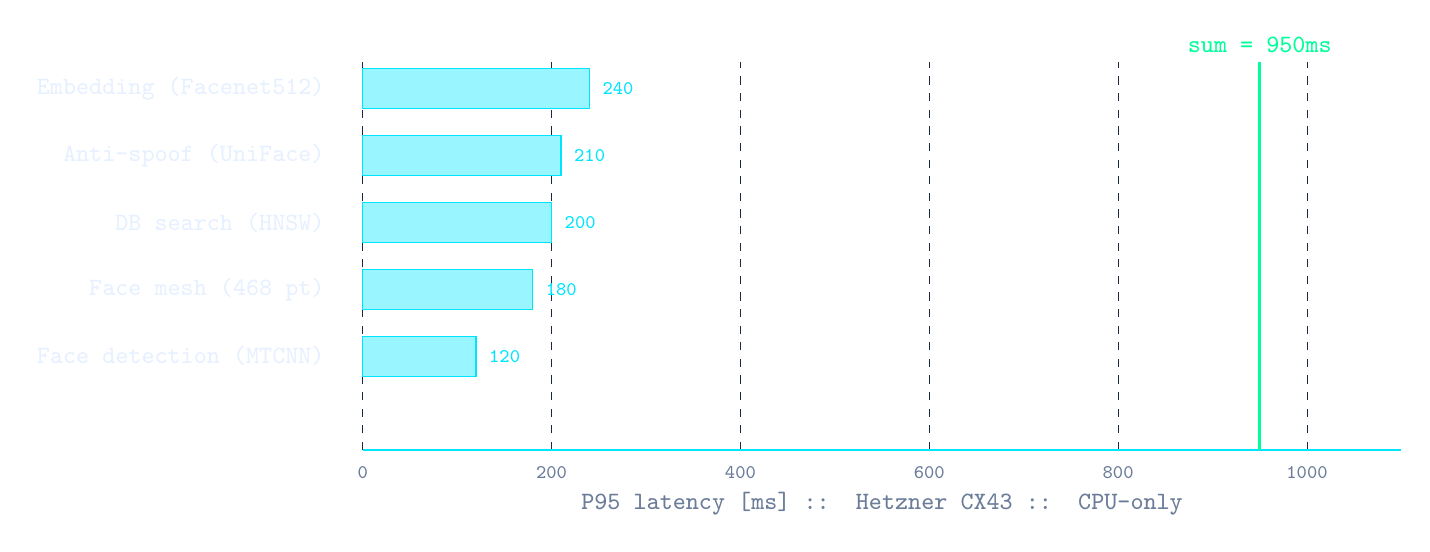
\begin{tikzpicture}[x=0.012cm, y=0.85cm,
  bar/.style={draw=CCyan, fill=CCyan!40, line width=0.5pt},
  axislabel/.style={font=\small\ttfamily, text=CInk, anchor=east},
  axislabelinside/.style={font=\scriptsize\ttfamily, anchor=west, text=CCyan},
  tickline/.style={CGrid, dashed, line width=0.3pt}]
\foreach \x in {0,200,400,600,800,1000}{
  \draw[tickline] (\x,-0.4) -- (\x,5.4);
  \node[font=\scriptsize\ttfamily, anchor=north, text=CDim] at (\x,-0.5) {\x};
}
\draw[CCyan, line width=0.5pt] (0,-0.4) -- (1100,-0.4);
\node[font=\small\ttfamily, text=CDim] at (550,-1.2) {P95 latency [ms] :: Hetzner CX43 :: CPU-only};
\node[axislabel] at (-30,5) {Embedding (Facenet512)}; \filldraw[bar] (0,4.7) rectangle (240,5.3); \node[axislabelinside] at (240,5.0) {\,240};
\node[axislabel] at (-30,4) {Anti-spoof (UniFace)};   \filldraw[bar] (0,3.7) rectangle (210,4.3); \node[axislabelinside] at (210,4.0) {\,210};
\node[axislabel] at (-30,3) {DB search (HNSW)};       \filldraw[bar] (0,2.7) rectangle (200,3.3); \node[axislabelinside] at (200,3.0) {\,200};
\node[axislabel] at (-30,2) {Face mesh (468 pt)};     \filldraw[bar] (0,1.7) rectangle (180,2.3); \node[axislabelinside] at (180,2.0) {\,180};
\node[axislabel] at (-30,1) {Face detection (MTCNN)}; \filldraw[bar] (0,0.7) rectangle (120,1.3); \node[axislabelinside] at (120,1.0) {\,120};
\draw[CGreen, line width=1.2pt] (950,-0.4) -- (950,5.4);
\node[font=\small\bfseries\ttfamily, text=CGreen, anchor=south] at (950,5.4) {sum = 950ms};
\end{tikzpicture}\par\vspace{2mm}

\setlength{\tabcolsep}{5pt}\renewcommand{\arraystretch}{1.15}\small\ttfamily
\begin{tabular}{@{}l r r@{}}
\textcolor{CDim}{quality\_metric}        & \textcolor{CDim}{target} & \textcolor{CDim}{observed} \\[1pt]
replay\_attack\_far (n=120)              & {<}\,1\%           & \textcolor{CGreen}{\bfseries 0.0\%} \\
passive\_spoof\_auc                      & {>}\,0.95          & \textcolor{CGreen}{\bfseries 0.97} \\
backend\_tests                           & green              & 633 / 633 \\
web\_vitest + playwright                 & green              & 619 + 27 \\
mobile (KMP) units                       & green              & 425 / 425 \\
\end{tabular}}

\block{\ttfamily [08] CONCLUSION}{%
\color{CInk}\small Production-grade, GDPR-compliant biometric auth \emph{is}
achievable on commodity hardware when the system is decomposed along its right
axis (OIDC contract vs.\ ML model) and when liveness is active, not just passive.
Measured 0\,/\,120 replay-attack false-accepts and a 0.97 passive-spoof AUC are
both within practical deployment limits on a single CPU server.}

\block{\ttfamily [09] FUTURE\_WORK[]}{%
\color{CInk}\small
\begin{itemize}[leftmargin=*, nosep, label=\textcolor{CCyan}{\ttfamily\bfseries >}]
  \item \textbf{BYOD tenant DB.} Enterprise tenants host biometric data in their own database, schema-pinned.
  \item \textbf{On-device pre-filter.} Stripped MediaPipe drops obvious non-faces before upload.
  \item \textbf{Cross-modal challenge.} Voice nonce + facial action to defeat audio-only deepfakes.
  \item \textbf{Verifiable credentials.} W3C VCs after successful KYC for downstream portability.
\end{itemize}}

\block{\ttfamily [10] DEMO :: REF}{%
\small
\begin{minipage}[t]{0.36\linewidth}\centering
\fcolorbox{CCyan}{white}{\qrcode[height=4.2cm,version=4,level=H]{https://verify.fivucsas.com}}\\[2mm]
{\ttfamily\color{CDim}\faCamera\ scan to test live demo}\\[1mm]
\ttfamily\bfseries\color{CCyan} verify.fivucsas.com
\end{minipage}\hfill\begin{minipage}[t]{0.62\linewidth}\footnotesize\color{CInk}\ttfamily
\textcolor{CMagenta}{// refs}
\begin{enumerate}[leftmargin=*, nosep, label=\textcolor{CDim}{[\arabic*]}]
\item Serengil, S., Özpınar, A. \textit{LightFace / DeepFace}. IEEE ASYU, 2020.
\item Lugaresi, C.\ et al. \textit{MediaPipe.} arXiv:1906.08172.
\item Soukupová, T., Čech, J. \textit{Real-Time Eye Blink Detection.} CVWW, 2016.
\item Wan, L.\ et al. \textit{Generalized End-to-End Loss for Speaker Verification.} ICASSP, 2018.
\item Yadav, S.\ et al. \textit{UniFace.} CVPR-W, 2023.
\end{enumerate}
\end{minipage}}

\end{columns}

% Footer ---------------------------------------------------------------------
\block[bodyinnersep=2mm, bodyverticalshift=0mm]{}{%
\colorbox{CBg}{\parbox{0.985\linewidth}{\centering\ttfamily
\vspace{2mm}\bfseries\small
\textcolor{CDim}{>>}\ \textcolor{CCyan}{\faGithub}\ \textcolor{CInk}{github.com/Rollingcat-Software/FIVUCSAS}
\quad\textcolor{CDim}{::}\quad
\textcolor{CCyan}{\faGlobe}\ \textcolor{CInk}{fivucsas.com}
\quad\textcolor{CDim}{::}\quad
\textcolor{CCyan}{\faEnvelope}\ \textcolor{CInk}{ahmetabdullahgultekin@gmail.com}
\quad\textcolor{CDim}{::}\quad
\textcolor{CCyan}{Marmara University \bfseries 2026}\vspace{2mm}}}}

\end{document}
